In this section I'll describe the model and the modifications I've made during second phase.
\subsection{The Model}
I chose a CNN, no other choice for that kind of task.
I started from a known network that I previously used for a similar task, comvbined with an intuition from a known model
for image classification.
I played a little with the number of filters for each layer, this way I can capture more features.
The problem with this method was that it take a lot of RAM (over 4GB), which made me debug on a pre-trained resnet18.
\begin{figure}[H]
    \centering
     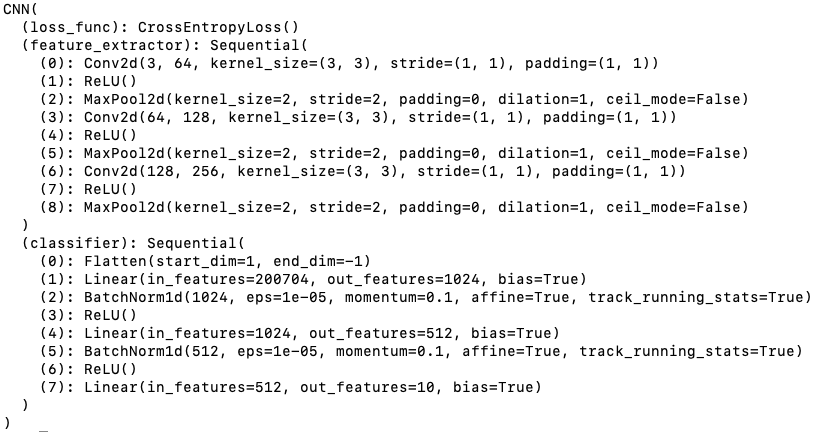
\includegraphics[scale=0.5]{images/architecture}
    \caption{architecture}
    \label{fig:architecture}
\end{figure}

\begin{figure}[H]
    \centering
    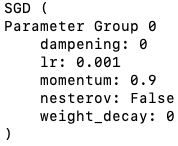
\includegraphics[width=0.25\textwidth]{images/optimizer}
    \caption{optimizer}
    \label{fig:optimizer}
\end{figure}

\subsection{Training}

\subsection{Testing Pipeline}
\begin{itemize}
    \item Take an image
    \item Determine if the object/s in the picture are human (using Human Detection Model model)
    \item Crop the object/s one by one (using first model), \& determine masked/non-masked/partially-masked (using second model)
\end{itemize}
